%  Synergies and mergers-Thursday, 19 November 2020
%
%  Created by Patrick on 2020-11-19.
%  Copyright (c) 2020 __Patrick Legros__. All rights reserved.
%
%!TEX encoding = UTF-8 Unicode  

\documentclass[a4paper,leqno]{article}%leqno to number equations on the left
\usepackage[utf8]{inputenc}
\usepackage{amsthm,amsmath,amssymb,amsfonts}
\usepackage{url}
\usepackage{hyperref}
\usepackage[round,longnamesfirst]{natbib}
%\bibliographystyle{plainnat}
\usepackage[mathscr]{euscript}
\let\euscr\mathscr \let\mathscr\relax
\usepackage[scr]{rsfso}
\usepackage{graphicx}
\usepackage{float}
\usepackage{enumerate}
\usepackage{blindtext}
\usepackage{setspace}
\usepackage{eurosym}
\usepackage{hyperref}
\usepackage{pdflscape}
\usepackage{array, multirow}
\usepackage[dvipsnames]{xcolor}
\usepackage{enumitem}
\usepackage{todonotes}

\usepackage{tikz}
\hypersetup{
colorlinks,
citecolor=NavyBlue,
linkcolor=NavyBlue,
urlcolor=NavyBlue}
\usetikzlibrary{matrix}
\newtheorem{prop}{Proposition}
\newtheorem{lemma}{Lemma}
\newtheorem{corollary}{Corollary}
\newtheorem{ass}{Assumption}
\newtheorem{result}{Result}
\newtheorem{condition}{Condition}
\newtheorem{Theorem}{Theorem}
\newtheorem{Definition}{Definition}
\newtheorem{remark}{Remark}
\newtheorem{example}{Example}

\newenvironment{reusefigure}[2][htbp]
  {\addtocounter{figure}{-1}%
   \renewcommand{\theHfigure}{dupe-fig}% If you're using hyperref
   \renewcommand{\thefigure}{\ref{#2}}% Figure counter is \ref
   \renewcommand{\addcontentsline}[3]{}% Avoid placing figure in LoF
   \begin{figure}[#1]}
  {\end{figure}}
  
  \usepackage{titlesec}

%\setcounter{secnumdepth}{4}

\titleformat{\paragraph}
{\normalfont\normalsize\bfseries}{\theparagraph}{1em}{}
\titlespacing*{\paragraph}
{0pt}{3.25ex plus 1ex minus .2ex}{1.5ex plus .2ex}

 \usepackage{geometry}

 
 \newcommand{\E}{\mathbb E}
 \newcommand{\N}{\mathcal N}
\renewcommand{\th}{\hat\theta}
\renewcommand{\t}{\theta}
\renewcommand{\a}{\alpha}
\renewcommand{\b}{\beta}
\newcommand{\s}{\sigma}
\newcommand{\de}{\delta}
\newcommand{\uut}{\underline{\underline{\theta}}}
\newcommand{\ut}{\underline{\theta}}
\newcommand{\uv}{\underline{v}}
\newcommand{\ov}{\overline{v}}
\newcommand{\up}{\underline{p}}
\newcommand{\op}{\overline{p}}


\begin{document}


\title{Data Driven Mergers and Information Synergies}
\author{Antoine Dubus and Patrick Legros\thanks{We would like to thank.}}
\date{\today}

\author{Antoine Dubus\thanks{~~Université Libre de Bruxelles, ECARES; \href{mailto:antoine1dubus@gmail.com}{antoine1dubus@gmail.com}.} $ $
Patrick Legros\thanks{~~Université Libre de Bruxelles, ECARES and CEPR; \href{mailto:patrick.legros@ulb.be}{patrick.legros@ulb.be}.}}

%\baselineskip0.7cm
\doublespacing

\maketitle


\begin{abstract}

\noindent Firms may share information to discover potential synergies. Information sharing modifies the competitive balance when firms compete head-to-head but may allow for more efficient mergers. We characterize equilibrium information sharing and we show that firms always benefit from sharing information, even if head-to-head competition has a positive probability of arising and the firm that shares information is made worse off than without information sharing. Because increasing information sharing both increases consumer surplus when there is head-to-head competition and when there is a merger, the presence of a regulator can decrease or increase the level of information sharing -- with a concomitant increase or decrease of consumer surplus -- with respect to the no-regulator case. A regulator who can also control the level of information sharing will allow firms to share information.
\end{abstract} 

JEL: G34; L86.

\textbf{Very preliminary, do not circulate.}

\newpage
\section{Introduction}


Mergers fail, claimed efficiencies at the time of merger review are often not realized, or if they are realized, they are not passed through to consumers. Is this because firms claim that the merger will yield efficiency gains in the hope of convincing authorities? Is it because firms haven't done their homework and incorrectly evaluated the extent of synergies? Or is it because synergies exist only ``on average'', hence that there is a probability that ex-post synergies may not exist?

These questions make sense in a world where firms are uncertain of the extend of synergies at the time they decide to merge. In such an environment, more precise information about the level of synergies that will follow a merger is valuable not only for the firms but also for the regulator. One way such an information can be generated is through information exchanges enabling firms to learn the synergistic value of two sets of data. While there is a value to information acquisition there are also costs: the information changes the competitive positions of the firms if the merger does not go through, but also changes the desire of a regulator -- who is aware of this information or can infer it from the decisions of firms to merge -- to allow the merger.

While our model could be applicable to collaborations like joint ventures, we will cast it in the context of data sharing and the complementarity of data and algorithms that two firms have developed. Important mergers and acquisitions have gone through in the past few years, which are motivated by the merger of data sets and algorithms in order to achieve information synergies. For instance, Facebook acquired WhatsApp to merge phone numbers with the profiles of Facebook users; Google is about to acquire Fitbit to complement the high precision profiles that Google has built thanks to its many online services with health data collected by the wearable devices sold by Fitbit.

Arrow famously pointed out the difficulty of inducing such collaborations among competitors, especially if what is shared is an idea that can be replicated at no cost. But even if there is a cost to replication, providing assets to competitors enhances their ability to compete, and sharing can be costly for the firm that shares its assets. Our contribution is to show that this competitive disadvantage is balanced by more efficient merger decisions, which is at the benefit of the firms, and sometimes of consumers.

Let us think for a minute of Google and Fitbit. Google does not have, yet, a competing product, nor has accumulated such data on users. Hence Fitbit has a significant competitive advantage on Google for wearable devices, at least a market leadership in the short term. The product value to consumers can be enhanced by leveraging the data that Google has accumulated into the algorithm developed by Fitbit, but this is not a certainty: the synergies between the data and algorithms of Google and Fitbit are yet unknown, even if both firms have a good understanding of the likelihood of these synergies. 

If Google obtains part of the data accumulated by Fitbit, it could develop its own product/algorithm and compete with Fitbit, weakening the competitive position of Fitbit if both firms compete head-to-head. We assume that the identity of the developer of the product is not neutral: a product developed by Google has the stamp ``Google'' on it, in particular inherits the concerns of consumers about privacy or the fact that the data collected by Google when they use this product will have effects on their web-surfing experience. Before developing a competing product, Google will have to explore the value it can bring to customers: this value is increasing in the level of data shared by Fitbit and the level of synergies $v$. Hence the more data Fitbit shares with Google, the weaker its competitive position. Because there is a cost to exploration, Google will engage in exploration only if sharing is large enough, and sharing is an investment that Fitbit does in order for Google and Fitibt to learn about their synergies.

If after exploration, synergies are learned to be low, a merger is not beneficial and Google and Fitbit will compete head-to-head, putting Fitbit in a worse situation than in the absence of sharing.\footnote{Hence, Google may need to give a transfer to Fitibt ex-ante to induce sharing.} But if synergies are high, a merger becomes beneficial and the new ``Google-Fitbit product'' is sold at a monopoly price, a better situation for Fitbit than in the absence of sharing. We characterize the optimal sharing level and show that while sharing will reduce the extend of inefficient mergers, it may not be able to do so perfectly: after sharing, the surplus when there is competition is lower than in the ex-ante stage, hence -- for a given synergy realization --  the total net surplus from a merger is higher after information sharing than without.


A regulator such as a competition authority should see with a keen eye information sharing practices. If synergies are high, sharing information will induce firms to merger, leading to a higher product quality and higher industry profits than without a merger. If synergies are low, competition between firms will be fiercer after information is shared, to the benefit of consumers. We show that the regulator has an impact on the amount of information shared by firms in equilibrium. On the one hand, if the regulator values competition between firms, the possibility that it prevents a merger increase with the amount of information shared, which reduces the incentives of firms to share information. On the other hand, the prospective buyer -- Google -- also has interest to acquire more information if there is a risk that the merger does not go through: with more information, it will achieve higher profits in the competitive case. 
todo relire ca

The remaining of this paper is organized as follows. We discuss the literature on mergers an acquisitions in Section \ref{lit}. We describe the model in Section \ref{model}, and we characterize the equilibrium in Section \ref{analysis}. Section \ref{regul} analyzes the impacts of a regulator on information sharing and social welfare. We consider bilateral information sharing in Section \ref{bilat}. Section \ref{disc} concludes.




\section{Literature}\label{lit}

Several reports have recently reconsidered competition policy for the digital era \citep{federico2019antitrust}. While \cite{scott2019committee} and \cite{shapiro2019protecting} call for a tightening of merger policy to fight abuses of dominant position, \cite{cabral2021merger} suggests caution in order not to discourage innovation. The role of data is central to this debate as  the success of digital companies is largely built upon the collection, use, sharing and sale of huge amounts of consumer data \citep{varian1989price, bergemann2015selling}. Data is a competitive asset \citep{hagiu2020data}, and because of the non-rival nature of information, firms are reluctant to share data with their competitors. As \cite{jones2020nonrivalry} argue, companies rather try to prevent competitors from accessing their data in order to keep a strong data competitive advantage over a market. The ability to secure exclusive access to high quality relevant data is viewed by many as a cause for the domination of digital markets by companies such as Facebook and Google. 

The literature thus sees information sharing between companies as a way to promote competition in digital markets \citep{martens2020business}.\footnote{Practices of information sharing have been well analyzed in economics \citep{vives1984duopoly, gal1986information}, and it is acknowledged that sharing information can have pro or anti competitive effects, in particular depending on the nature of competition (cournot vs bertrand).} \cite{tirole2020competition} and \cite{cremer2019competition} among others suggest to ensure fair and equal access to information between firms following FRAND licensing terms.\footnote{This suggestions also echoes \cite{admati2000forcing} who analyze the importance of the disclosure of financial information by firms.} By doing so, firms would equally access data and compete on a level playing field. 



In a race to data dominance, digital companies have engaged in an important merger wave. Mergers are now data driven, and recent articles have analyzed how acquiring a firm's data set has become a motivation for mergers and acquisitions \citep{stucke2016introduction}. For instance, the European Commission investigated whether information synergies were possible in the acquisition of WhatsApp by Facebook \citep{argentesi2019merger}.\footnote{Facebook lied to the Commission by claiming that data sets owned by the two companies were impossible to merge, and the Commission eventually fined Facebook for concealing the potential for information synergies of the merger (\href{https://ec.europa.eu/commission/presscorner/detail/pl/IP_17_1369}{Commission fines Facebook €110 million for providing misleading information about WhatsApp takeover, last accessed 04/12/2021}).} More recently, the European Commission gave its green light for Google to acquire Fitbit under the condition that data from both companies would not be merged, as it would result in information synergies that may end up harming consumers. Additionally, Microsoft has recently been pointed out for willing to acquire the large consumer base of Discord, and the related consumer data.\footnote{\href{https://www.lemonde.fr/economie/article/2021/04/08/microsoft-convoite-le-service-de-discussion-discord_6076070_3234.html}{Microsoft/Discord}} 



Synergies resulting from mergers and acquisitions have been extensively studied in the literature.\footnote{\cite{damodaran2005value} reviews different types of synergies considered in the literature and assesses what issues can emerge from misperceptions of the benefits from different synergies.} \cite{chatterjee1986types} distinguishes three types of synergies: financial, operational, and collusive. He shows that collusive synergies are associated with the highest value from a merger, while operational are associated with the lowest values. Nevertheless, \cite{mukherjee2004merger} report that operational synergies are given by firms as the main reason to merge. \cite{gupta2002quantifying} quantify operational synergies and highlight the importance of production characteristics of the acquirer and of the target for synergies to arise. \cite{larsson1999integrating} highlight the importance of common culture between two companies for a merger to succeed. They show that synergy realization is a function of the similarity and complementarity of the two merging businesses, and of the extent of interaction and coordination during the organizational integration process. \cite{madura2008clustered} shows that the valuation of synergies by companies and markets is based on synergies measured in recent takeover in the same industry.

The above literature does not consider information synergies, probably because data has become essential for many business models only recently. Our approach can be seen as a natural followup of these studies, as information synergies naturally arise depending on the complementarity of data sources. As data is becoming an essential facility in a fast-growing number of industries, it is important to understand the role of information synergies in mergers and acquisitions. A firm has incentives to learn the potential for complementarity before engaging a data driven merger, and we will show how information sharing can be used by firms to assess information synergies.


The literature on information theory has for long acknowledged the importance of information synergies. A recent trend of the literature has focused in particular on quantifying unique, redundant, and synergistic information when considering two data sets. For instance, \cite{bertschinger2014quantifying}, \cite{Griffith2014}, and \cite{olbrich2015information} discuss how information synergies can arise when merging two data sets. This literature is the theoretical starting point of our interest for information synergies during mergers. Moreover, \cite{sootla2017analyzing} empirically measure the synergistic coefficient of two data sets. This last paper will support several hypothesis that we use in our model. In particular, it justifies that synergies are learned when data sets are merged. 


\medskip

This paper is closely related to the literature on the sale of technology. \cite{d2000bargaining} focus on a problem in which a seller can disclose verifiable knowledge that is used for contracting. \cite{anton2002sale} analyze how an inventor can disclose part of its innovation to a prospective buyer in order to reveal its quality. We adopt the common view that shared information can be used by the receiver to compete with the sender, following the well known Arrow information paradox. However, our paper differs from the literature on licensing as we consider both firms endowed with data and uncertain synergies, and we are interested in the synergistic value from combining both data sets. 

\medskip

Our paper also relates to the relation between market competition and firms' incentives to merge, which has been under the spotlight of competition authorities for several decades now, and has been recently reignited by concerns over so called killer acquisitions \citep{cunningham2021killer}. \cite{kamepalli2020kill} and \cite{shelegia2021kill} show that such killer acquisition do not necessarily foster innovation and competition through more market entry. Contrary to the standard view of this literature, competition in our approach won't be used as a motivation for a firm to merge, but will be used by the acquirer to lower the profits of its target, and in turn to lower the price of the acquisition.

Finally, a recent literature has also analyzed the competitive impacts of data driven mergers.\footnote{\cite{chirita2018data} calls for accounting for potential privacy loss when assessing the impacts of data driven mergers.} \cite{de2020data} characterize when data is pro or anti competitive. \cite{chen2020data} show that data driven mergers increase consumer surplus as long as there are still competitors in the market. These articles focus on the consequences of a mergers, assuming perfect information on the outcome of the merger. By contrast, we argue in this article that such assumption is in general not satisfied, and that merger participants usually do not know for sure the extend of their complementarities, in particular regarding information synergies. They can discover this synergistic value and take better merger decisions by sharing information before the merger takes place.


%TBD: Optimal merger policy when firms have private information \cite{Besanko1993}.

%Startups and upstarts \cite{awaya2021startups}.


\section{Model}\label{model}


We consider two firms, indexed by $1,2$, where $2$ is a dominant firm (Google) and $1$ is a firm that has developed a new product of platform (Fitbit) and has a stock of data of mass $1$ generated by this activity. Firm $1$ is able to give a utility level of $u$ to its customers and absent other competition can fix a price equal to $u$, making a profit of $u$ (assume a mass one of customers interested by the product.)


Firm $2$ has developed other products and has its own stock of data. Combining data from $1$ and $2$ will enhance the value to customers to $v\in\{\uv,\ov\}$. The value of $v$ is unknown to firms, but each firm knows that $v=\uv<u$ w.p. $\a$, and $v=\ov>u$ w.p. $1-\a$. 


If firm $1$ does not share data, a merger may happen but it will be under imperfect information. If firm $1$ shares data with firm $2$, firms will learn the value of the synergies and they will merger if synergies are high, therefore avoiding low valuation mergers. Treating data to identify and generate synergies is costly, and we denote by $e$ this cost. This data exploitation cost corresponds for instance the development of new algorithms or code, or to further marketing efforts. 


Firm $1$ can share $s\%$ of its data with firm $2$, possibly at an agreed upon price $T(s)$: at this time of sharing, firms $1,2$ do not know the value of $v$, but they know that $v=\uv$ with probability $\a$ and $v=\ov$ with probability $1-\a$. Upon receiving $s$, firm $2$ can either exerts effort $e$ at cost $-e$, in which case the synergy $v$ is learned with probability $1$ if $e\geq C(s)$, and with probability zero otherwise. To simplify, synergies are learned by both firms, the case where firm $2$ gets this information privately is addressed in an extension. When synergies are known, firms and consumers know that the product provides value $v s$ to customers if a share $s$ of the data of firm $1$ is used.\footnote{We assume that consumers always know the value of a product as soon as it is on the market.} 


If $v$ is known, Firm 2 can then make a TIOLI offer to firm $1$ for creating a merger, or can choose to use the information to compete with firm $1$. If there is a merger customers will have value $v$ (since all data from firm $1$ is part of the assets of the merged firm). If firms do not merge, firm $2$ has a product providing value $vs$ to customers, and that it can use to compete with firm $1$.

Exploitation cost $C(s)=c\cdot(1/s-1)$ decreases with $s$: $c\geq 0$, $c(1)=0$, $c(0)=+\infty$, and $c'(0)=-\infty$. This cost function captures the idea that one can always do at least as good with more data than with fewer. With $\epsilon$ data, it is infinitely costly to learn $v$. In equilibrium firm 2 will either invest $e=C(s)$ and learn the value of the synergy, or not invest and remain uninformed.


A regulator can allow or prevent the merger, in order to maximize a social welfare function finding a tradeoff between consumer surplus weighted by $\rho\in[0,1]$ and industry profits weighted by $1-\rho$. In particular, when $\rho=1$, the regulator protects consumer surplus and does not account for the profits of the industry. On the contrary, when $\rho=0$, the regulator only accounts for the profits of the industry when deciding to allow or prevent the merger. 


At the time firms ask for approval of the merger, they do know for sure what will be the decision of the regulator. For instance when Google makes an offer to acquire Fitbit, it is not clear what will be the decision of a competition authority: the merger will increase product quality and industry profits, but firms will compete fiercely if the merger is prevented, increasing consumer surplus. The decision of the regulator balances these two effects depending on the value of $\rho$, and we assume that firms do not know this value before the regulator takes a decision. This uncertainty is resolved only at the time the regulator evaluates the merger proposal, that is after $s$ has been shared and firms engage in a merger. We assume that, after firms have asked to merge, the regulator observes a draw $\rho$ from a uniform distribution on $[0,1]$. Additionally, we will analyze whether the regulator wants to allow or forbid pre-merger information sharing. We will show that information sharing changes the intensity of competition in case the merger is prevented, and thus that it changes the decision of the regulator to allow or prevent the merger.
todo relire toute cette partie


The timing of the game is the following:


\begin{itemize}[label={-}]
    \item Stage 1: firm 2 either remains uninformed, or purchases $s$ information from firm 1 for transfer $T(s)$, invests $e=C(s)$ and learns $v$.
    \item Stage 2: firm 2 makes a take it or leave it offer to acquire firm 1. If firm 1 declines the offer, firms compete.
    \item Stage 3: firms go to the regulator to have the merger allowed, the regulator learns $\rho$ and decides to allow or prevent the merger.
    \item Stage 4: depending on the regulator's decision, firms compete or merge and make profits.
\end{itemize}


The following hypothesis are important elements of the analysis:

\begin{itemize}[label={-}]
    \item H1: when a product is on the market, consumers know their valuation immediately. This holds even if firms do not know the quality of the product at the time they launch it. 
    \item H2: $u\geq 2\uv$ and $\a\uv\geq1$.
    \item H3: product quality can decrease after a merger: $\uv\leq u$
\end{itemize}



Assumption H1 is supported by the important literature on pricing of information goods \citep{shapiro1998information} that shows how consumers have access to many ways to discover their valuation of a product before acquiring it, through sampling, free downloading, freemium, rating and reviews. Beyond realism, the assumption allows us to avoid asymmetries of information at the product market stage.

Assumption H2 insures that, under perfect information, firm 2 will engage in a merger only with type $\ov$. The extension to situations where it is also profitable for firm 2 to acquire firm 1 when synergies are low is straightforward and preserves our qualitative results.

In Assumption H3 we posit that when firm 2 purchases firm 1, it may not be able to sell the product at the same value than if the merger did not go through. We rationalize this assumption by the branding value of the name. For instance, many WhatsApp users migrated to privacy preserving apps such as Signal and Telegram after the company updated its terms of services to share user data with Facebook, its parent company. \footnote{\href{https://www.cnbc.com/2021/01/18/whatsapp-delays-privacy-update-amid-facebook-data-sharing-confusion.html}{WhatsApp delays privacy update over user ‘confusion’ and backlash about Facebook data sharing, CNBC, last accessed June 2, 2021}.} This change of the value of a product after an acquisition is supported by the management and economics literature on brand reputations \citep{fombrun1990,tadelis1999s}, or the fact that mergers may be accompanied by re-branding of products.

\section{Analysis}\label{analysis}

We first analyze the incentives of firm 2 to purchase information from firm 1 in the absence of a regulator. We show that information sharing allows firm 2 to avoid merging when synergies are low, and, in equilibrium, information sharing is always more profitable for firm 2 than merging under imperfect information.

\subsection{Competition}


Suppose that firm $1$ shares $s>0$, and let us ignore for the moment the possibility of a merger. If firm $2$ invests $C(s)$ and learns $v$, it can provide its customers a value $vs$ while firm $1$ can provide a value $u$. Assuming Bertrand competition the equilibrium price paid by the consumers and the profit per consumer are

\begin{align}\label{comp}
\begin{cases}
    p=vs-u,\; \pi_1(v,s)=0,\; \pi_2(v,s)=vs-u & \text{ if }vs-u\geq 0\\ 
    p=u-vs\; \pi_1(v,s)=u-vs,\; \pi_2(v,s)=0 & \text{ if }vs-u\leq 0.
\end{cases}
\end{align}

If firm $2$ does not invest, its profit per consumer is equal to zero, that of firm $1$ is equal to $u$ and synergies are not learned.


\subsection{Merger}
%
Suppose that no data is shared. A merged firm has access to the full stock of data $s=1$ that it can exploit at cost $C(1)=0$. Therefore, the expected value if there is investment is $\E[v]=\a \uv+(1-\a)\ov$.

It is useful to introduce the notion of ex-ante efficiency. A merger is ex-ante efficient if $\E[v]\geq u$ and it is ex-ante inefficient when $\E[v]\leq u$. It is clear that without information, firm 2 will acquire firm 1 only when the merger is ex-ante efficient. 


Because $\uv<u$, the merged firm over-invests when $v=\uv<u$. On the contrary, firms expect high synergies to take place with some probabilities and $\ov>u$. This explains why information sharing can allow firms to merge, even in cases where mergers are ex-ante inefficient, as we will show in Proposition \ref{prop:1}. 

\subsection{Profits with data sharing}

Suppose firm $1$ shares $s$ with firm $2$, and that firm $2$ agrees to pay $T(s)$ to firm $1$ for this amount of data. 

Upon receiving $s$, firm $2$ can decide to invest $C(s)$ in order to learn $v$. In this case, the two firms anticipate payoffs $\pi_i(v,s)$ as given by \eqref{comp} if there is no merger. Firm $2$ can make a TIOLI offer to buy firm $1$'s asset at a price $p(v,s)$ that will make firm $1$ indifferent between merging and not merging, that is 
%
\begin{equation}\label{merger-price}
    p(v,s):=\pi_1(v,s).  
\end{equation}
%

When $s\leq \frac{u}{\ov}$, firm 1 makes positive profits when firms compete, regardless of the value of $v$. Firm 2 exerts a competitive pressure on firm 1, and to compensate for this loss of profits, it has to pay $T(s)=\E[v]s$ to acquire information $s$. Firms merge only when $v=\ov$, and the price of the acquisition corresponds to the profits of firm 1 when firms compete: $p(\ov,s)=u-\ov s$.

But when $\frac{u}{\ov}\leq s$ and firms compete, firm 1 makes positive profits if $v=\uv$, and makes zero profits if $v=\ov$. Hence, to compensate for this loss, firm 2 must pay $T(s)=u-\a(u-\uv s)$ to firm 1 to acquire information. Firm 2 wants to merge only when $v=\ov$ and as in this case, firm 1 makes zero profits in the competitive set-up, firm 2 can acquire firm 1 at a zero price.


Lemma \ref{lem1} gives the price $T(s)$ paid by firm 2 for information as well as the price of the acquisition when firm 2 invests $C(s)$ following sharing of data and learning $v$ (all proofs absent from the text are in the Appendix).

\begin{lemma}~~\label{lem1}

The price of information, and the price firm 2 pays to acquire firm 1 are: 

\begin{itemize}
    \item When $s\leq \frac{u}{\ov}$:
    $$T(s)=\E[v]s~~and~~p(\ov,s)=u-\ov s.$$ 
    
    \item When $\frac{u}{\ov}\leq s$:
    $$T(s)=u-\a(u-\uv s)~~and~~p(\uv,s)=0.$$
 \end{itemize}

\end{lemma}

\noindent The price firm 2 pays to acquire firm 1 after the synergies are learned decreases with $s$. For $s\geq\frac{u}{\ov}$, firm 2 can sell a better product than firm 1 if firms compete, firm 1 makes zero profits and is indifferent between competing or being acquired at a zero price. Thus the price $T(s)$ of information increases with $s$, as firm 1 expects lower revenues when sharing more information with firm 2.

\medskip

Lemma \ref{lem2} provides the expected profits of firm 2 when purchasing $s$ information from firm 1 at the beginning of the game. 

\begin{lemma}~~\label{lem2}

The expected profit of firm 2 purchasing information $s$ from firm 1 is:

    $$\pi_2(s)=(1-\a)(\ov -u)-\a \uv s-C(s).$$ 

\end{lemma}

\noindent More information shared has two opposite effects on the profits of firm 2. On the one hand, more information is costly to acquire from firm 1, which lowers the profits of firm 2. On the other hand, more information also decreases the data exploitation cost $C(s)$ and increases the profits of firm 2. We characterize in the next section the optimal amount of information shared, which balances these two opposite effects of information acquisition on the profits of firm 2.


\medskip

\subsection{Information acquisition}\label{infacq}

We analyze when it is profitable for firm 2 to purchase information from firm 1, and we characterize optimal information sharing. The alternative for firm 2 is not to purchase data, and to merge under imperfect information. In this case, firm $2$ makes a TIOLI offer to buy firm $1$ at price $u$ and firm $2$ makes profit $\E[v]-u$. 


We show that the optimal sharing can dominate no sharing for firm $2$. To obtain the equilibrium amount of information shared by firm 1 we apply first order conditions with respect to $s$ on the profit of firm 2 with information $s$: $\pi_2(s)=(1-\a)(\ov -u)-\a \uv s-C(s)$. In equilibrium, $s^*$ satisfies $\a \uv =-C'(s^*)$, or, given our assumption on $C(s)$:

\begin{equation}
    s^*=\min\left\{1,\sqrt{\frac{c}{\a \uv}}\right\}.
\end{equation}


\noindent When $c$ decreases, the data exploitation cost decreases as well and the benefits for firm 2 of lowering the cost by purchasing more information decrease.

\medskip

We now compare profits with and without information sharing and we show that firm 2 prefers to purchase information before merging.

\begin{prop}~~\label{prop:1}

\begin{itemize}
    \item (a) When $E[v]\geq u$ information sharing is always optimal.
    \item (b) When $E[v]\leq u$ there exists $\tilde{c}$ such that firms share information if and only if $c\leq \tilde{c}$.
\end{itemize} 

\end{prop}

\noindent Proof: see Appendix \ref{prop:1p}.

\medskip

\noindent Proposition \ref{prop:1} is an important contribution of this article. When $E[v]>u$, mergers are ex-ante efficient and firms always benefit from information sharing. Information allows firms to learn the value of synergies, and to avoid merger when synergies are low. 

\medskip

By contrast, when $E[v]<u$, information sharing is profitable if $\pi_2(s)=(1-\a)(\ov -u)-\a \uv s-C(s)\geq0$. The profitability of partial information sharing thus depends on the level of the data exploitation cost. If the data exploitation cost is high, firm 2 does not exploit data and, as mergers are ex-ante inefficient, firms do not merge. On the contrary, if $C(s)$ decreases quickly, partial information sharing is more profitable than not merging, and information sharing allows ex-ante inefficient mergers to take place

\medskip


\section{The Regulator's Problem}\label{regul}

We consider now a regulator who decides whether to allow or prevent the merger. The regulator maximizes a social welfare function that weights the social cost of high industry profits and the social benefit of synergies. Contrary to the usual view that synergies are created only during the merger, synergies endogenously happen without a merger if firm $1$ shares some of its data with firm $2$. Hence, when evaluating a merger proposal, the regulator will compare the \emph{relative industry gain} weighted by $1-\rho$ to the \emph{relative gain of consumer surplus} weighted by $\rho$.

\medskip

The total profit of the industry is equal to $u$ if there is no information sharing and no merger, to $max\{u-v s,v s-u\}$ if firm 2 has information $s$ and firms compete, and to $v$ if firms merge.

\medskip

Consumer surplus is equal to zero if a firm is a monopoly and there is full surplus extraction. This case takes place when there is no information sharing and no merger, and firm 1 is a monopolist, or when firm 2 acquires firm 1. On the contrary, if information has been shared and firms compete, consumer surplus is equal to $\min\{u,v s\}$.

\medskip


\subsection{Merger decision without information sharing}

We analyze the decision of the regulator with draw $\rho$ to allow or prevent a merger when no information has been shared. In this case, consumer surplus does not change as competition never occurs, and only the gains of the industry are considered: $(1-\rho) (v-u)$.

For $v=\ov\geq u$, without information sharing merger is always beneficial from the regulator's point of view: since firms do not compete, there is no loss of surplus for consumers, and there is a social benefit from synergy gains. Now, for $v=\uv$, without information sharing a merger is never beneficial from the regulator's point of view. Hence, without information sharing, there is imperfect information on $v$ and the regulator allows the merger if $\E[v]\geq u$ and prevents it if $\E[v]\leq u$.

\medskip

\subsection{Social welfare with information sharing}

\medskip

At the time the regulator has to evaluate a merger, firm $1$ has already shared $s$ with firm $2$ and both firms and the regulator know the value of $v$. If $v=\uv$, firm 2 does not propose to merge and exerts a competitive pressure on firm 1. If $v=\ov$, under competition firms lower their prices providing consumers with surplus equal to $\min\{u,\ov s\}$, which is lost to consumers if the regulator allows the merger. On the other hand, the industry gain is $(1-\rho) (\ov-\max\{u-\ov s,\ov s-u\})$. Hence the welfare gain from the merger is

%

\[
(1-\rho) (\ov-\max\{u-\ov s,\ov s-u\})-min\{u,\ov s\}\rho
\]

Lemma \ref{lem3} characterizes the probability that a merger is authorized, and the expected payoff of firm 2 when acquiring information from firm 1.

\begin{lemma}~~\label{lem3}

\begin{itemize}
    \item There exists a decreasing function $\rho^*(s)$ such that the regulator authorizes the merger if, and only if, $\rho\leq \rho^*(s)$. 

Hence, as we consider $\rho$ following a uniform distribution over $[0,1]$, the probability of a merger is $\rho^*(s)$.
    \item The function $\rho^*(s)$ depends on whether $s\in[0,\frac{u}{\ov}]$ or $s\in[\frac{u}{\ov},1]$, and we have: 

\begin{align}
~\rho^*(s)=
\begin{cases}
    ~~\frac{\ov(1+s)-u}{\ov(1+2s)-u}~~\textrm{if}~s\in[0,\frac{u}{\ov}]\\ 
    ~~\frac{\ov(1-s)+u}{\ov(1-s)+2u}~~\textrm{if}~s\in[\frac{u}{\ov},1].
\end{cases}
\end{align}
    \item The expected payoff of firm 2 when purchasing $s$ information from firm 1 is:
    
\begin{align}
~\pi_{2r}(s)=
\begin{cases}
    ~~(1-\a)\rho^*(s)(\ov(1+s)-u)-\E[v]s-C(s)&\textrm{if}~s\in[0,\frac{u}{\ov}]\\ 
    ~~(1-\a)[\rho^*(s)\ov+(1-\rho^*(s))(\ov s-u)-u]-\a\uv s-C(s)~~&\textrm{if}~s\in[\frac{u}{\ov},1].
\end{cases}
\end{align}
\end{itemize}

\end{lemma}

\medskip

\noindent The probability $\rho^*(s)$ that a merger is allowed decreases with $s$ as more information sharing implies that firms compete more fiercely, which benefits consumers. The opportunity cost of a merger is thus larger for higher values of $s$ and a merger is beneficial only if $\rho$ is large enough. 

\medskip

Information sharing can lead the regulator to prevent ex-ante efficient mergers ($\E[v] \geq u$) when $\rho \geq \rho^*(s)$, as without merger, firms compete, which benefits consumers through an increase of their surplus. 

\medskip

\subsection{Information acquisition}

We analyze how the presence of the regulator and the possibility that it prevents the merger impact the incentives of firm 2 to purchase information from firm 1. There are two opposite effects of the regulator on the incentives of firms to share information. On the one hand, the possibility that the regulator prevents a merger increases with the amount of information shared, which reduces the incentives of firms to share information. On the other hand, firm 2 has interest to acquire more information in case the merger does not go through: with more information, firm 2 will achieve higher profits in the competitive case. 

In order to analyze the impacts of the regulator on the amount of information shared in equilibrium, Lemma \ref{lem5} provides condition on the data exploitation cost for the expected payoff of firm 2 to be strictly concave when there is a regulator. 

\begin{lemma}~~\label{lem5}

There exists $c_{c}$ such that when $c>c_{c}$, $\pi_{2r}(s)$ is strictly concave on $[0,\frac{u}{\ov}]$ and on $[\frac{u}{\ov},1]$.

\end{lemma}

\noindent Proof: see Appendix \ref{lem5p}

\noindent In the remaining of the analysis, we focus on $c>c_{c}$ such that the expected payoff of firm 2 when purchasing information is strictly concave on each interval. The concavity of $\pi_{2r}(s)$ over the two distinct intervals $[0,\frac{u}{\ov}]$ and $[\frac{u}{\ov},1]$ implies that there are several shapes of the profit functions to consider. From the analysis of function $\pi_{2r}(s)$ provided in Appendix \ref{lem5p}, we can characterizes thresholds values $c_0,c_1,~\&~c_2$ that distinguish intervals of $c$ for which $\pi_{2r}(s)$ is monotonously increasing or decreasing, or has a unique interior maximum. 

\begin{lemma}~~\label{lem7}

There exist $c_0,c_1,~\&~c_2$ such that:

\begin{itemize}
    \item On interval $[0,\frac{u}{\ov}]$:
    \begin{itemize}
        \item $\pi_{2r}(s)$ has a unique maximum when $c\leq c_1$;
        \item $\pi_{2r}(s)$ is strictly increasing when $c\geq c_1$.
    \end{itemize}
    \item On interval $[\frac{u}{\ov},1]$:
    \begin{itemize}
        \item $\pi_{2r}(s)$ is strictly decreasing when $c\leq c_0$;
        \item $\pi_{2r}(s)$ has a unique maximum when $c\in[c_0,c_2]$;
        \item $\pi_{2r}(s)$ is strictly increasing when $c\geq c_2$.
    \end{itemize}
\end{itemize}

\end{lemma}

\noindent Proof: see Appendix \ref{lem5p}.

\noindent The different cases depending on the value of $c$ are summarized in Figure 1 when $c\leq c_2$ and in Figure 2 when $c\geq c_2$. Note that as $C'(0)=-\infty$, $\pi_{2r}(s)$ is never monotonously decreasing on $[0,\frac{u}{\ov}]$. Moreover, when $c_0\leq c\leq c_1$ the global maximum can belong to $[0,u/\ov]$ or to $[u/\ov,1]$. 

\medskip

\begin{figure}[H]
\leftskip -0,5cm{
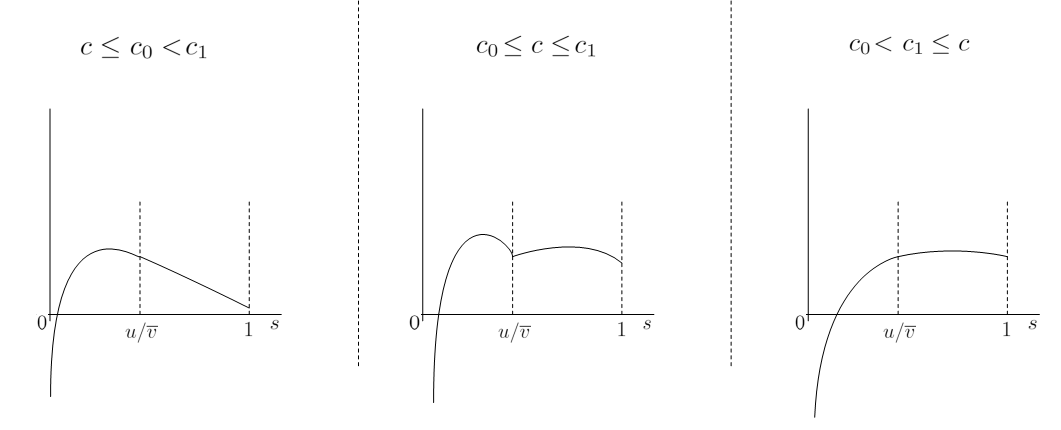
\includegraphics[scale=0.55]{Figure1}
\caption{Profits with regulator: $c<c_2$, interior solutions}\label{Figure1}}
\end{figure}


\begin{figure}[H]
\leftskip 1,5cm{
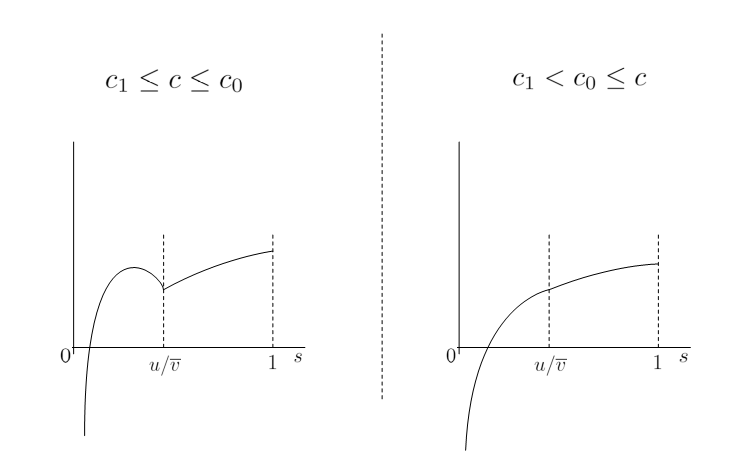
\includegraphics[scale=0.55]{Figure2}
\caption{Profits with regulator: $c>c_2$, corner solutions}\label{Figure2}}
\end{figure}

\medskip

The data exploitation cost is key to understand the effect of the regulator on information sharing. Low exploitation costs will make it less profitable to share more information, and firm 2 will optimally purchase $s\in[0,\frac{u}{\ov}]$. High exploitation costs will give incentives to firm 2 to purchase more, and we show in the next section that it will add a new effect to information sharing: in case the merger is declined, the higher the $s$ the higher the profits of firm 2 under competition.

\medskip

Let us look at the last case, where the profit of firm 2 is maximized for $s=1$. Replacing $s$ by $1$ in the profit of firm 2 given in Lemma \ref{lem3} we obtain:

$$\pi_{2r}(s)=(1-\a)\ov-\a\uv-\frac{3}{2}(1-\a)u.$$

Profits are positive for sufficiently high values of $\ov$. We can show that it is profitable for firm 2 to purchase information instead of merging under imperfect information and have an expected payoff of $\E[v]-u$. Comparing profits in both cases, sharing information is more profitable than merging under imperfect information when:

\begin{equation}\label{eq2}
    u(3\a-1)\geq 4\a\uv.
\end{equation}

This inequality is satisfied under two conditions: $3\a\geq1$; and $\frac{u}{\uv}\geq \frac{4\a}{3\a-1}$. These two conditions imply that there is a sufficient expected loss from merging under imperfect information, so that sharing information allows to avoid this loss.

\medskip

\subsubsection{Does the presence of the regulator drive up or down consumer information sharing?}

We compare information sharing in equilibrium with and without the regulator. We replace $s$ by $s^*$, the optimal amount of information shared without a regulator, into $\pi_{2r}(s)$ and we see whether the profit of firm 2 with the regulator increases or decreases  at $s^*$. This allows us to show whether more or less information is shared when there is a regulator. 

todo voir comment faire "this should be earlier"

\begin{prop}~~\label{prop:2}

Let's $s_r^*$ denote the optimal value of $s$ with the regulator. there exists a value $\underline{c}$ of the data exploitation cost such that:

\begin{itemize}
    \item When $c\leq\underline{c}$: $s_r^*\in[0,u/\ov]$ and the presence of the regulator reduces the amount  of information shared in equilibrium:
    
    $$s_r^*<s^*.$$
    \item When $c>\underline{c}$: $s_r^*\in[u/\ov,1]$ and the presence of the regulator increases the amount of information shared in equilibrium:
    
    $$s_r^*>s^*.$$
\end{itemize}

\end{prop}

\noindent Proof: see Appendix \ref{prop:2p}.


\noindent There are two cases to consider to understand to impact of the regulator on pre-merger information sharing. When $s_r^* < u/ \ov$, more information shared decreases the exploitation costs but lowers the probability that the merger is accepted. In this case, firm 2 purchases \textit{less} information from firm 1 than without the regulator. 

\medskip

When $s_r^*> u/ \ov$ there is an additional positive effect of information sharing on the profits of firm 2: if the merger is prevented, the larger $s$ is, the higher the profits of firm 2 under competition. With a uniform distribution this second effect dominates the first effect on the interval $[u/\ov,1]$, and firm 2 purchases \textit{more} information than without a regulator. 

\medskip

We illustrate these cases where $s_r^*\in[0,u/\ov]$ and $s_r^*\in[u/\ov,1]$ in a numerical example. Consider $\a=\frac{3}{4}$, $\ov=4u=8\uv=1280$. Clearly in this example the condition given in Eq. \ref{eq2} for information sharing to be more profitable than non sharing is satisfied as $u(3\a-1)\geq 4\a\uv$, and the profit function is strictly concave on $[0,u/\ov]$ and on $[u/\ov,1]$ for $c>\underline{c}=5.76$. In this case, $c_0=6.7$, $c_1=21.1$ and $c_2=40$. For $c\in[5.76,6.7]$, $\pi_{2r}$ has a unique maximum $s_r^*\in[0,u/\ov]$, and there is less data sharing than without the regulator. For $c\geq21.1$, $\pi_{2r}$ has a unique maximum $s_r^*\in[u/\ov,1]$ and firm 2 collects more data than without the regulator. In particular, when $c\geq 40$ $s^*_r=1$ and firm 1 shares all information. 

todo verifier les valeurs numériques

\medskip

The cost function determines whether it is more profitable for firm 2 to purchase more or less information than without the regulator. When data exploitation costs are low, firm 2 has interest to purchase a smaller amount of data than without the regulator, while when costs are high, firm 2 purchases more information. This stresses the importance of the data exploitation cost - and thus of the data exploitation capacities of firms - for the efficiency of mergers. In particular, we analyze in the next section how sharing more or less information impacts consumer surplus when the merger is prevented.

\medskip

\subsubsection{The impact of the regulator on consumer surplus.}

We now analyze the impact of the regulator on consumer surplus, which goes through two effects. On the one hand, firms can share more or less information with than without the regulator. When more information is shared, consumer surplus is higher in case synergies are low and firms compete. On the other hand, the regulator can also prevent the merger when synergies are high, in order to make firms compete and keep a high level of consumer surplus. 

\medskip

The first effect depends on the optimal amount of information shared by firm 1. If firm 2 purchases $s_r^*\in[u/\ov,1]$ data, $s_r^*>s^*$ and consumer surplus is equal to $\a \uv s_r^*+(1-\rho^*(s_r^*))u>\a \uv s^*$. The second effect go in the same direction as the first, and in this case the presence of the regulator always increases consumer surplus. 

\medskip

If firm 2 purchases $s_r^*\in[0,u/\ov]$ data, $s_r^*<s^*$ and consumer surplus is equal to $\a \uv s_r^*+(1-\rho^*(s_r^*))\ov s_r^*$. The second effect goes in the opposite direction, and in this case the presence of the regulator has an ambiguous effect on consumer surplus. Proposition \ref{prop:3} summarizes this discussion.


\medskip

\begin{prop}~~\label{prop:3}

\begin{itemize}
    \item When $s_r^*\in[0,u/\ov]$:
    \begin{itemize}
        \item When synergies are low, firms compete and consumer surplus is lower than in the no-regulator case.
        \item When synergies are high and the merger is prevented, consumer surplus is higher than in the no-regulator case.
    \end{itemize}
    \item When $s_r^*\in[u/\ov,1]$ the presence of the regulator always increases consumer surplus.
\end{itemize}

\end{prop}

\noindent The ambiguous effect that the regulator can have on consumer surplus comes from the fact that the regulator maximizes social welfare accounting for the profits of the industry on top of consumer surplus. When the data exploitation cost is higher that $\underline{c}$, firms share more information and consumer surplus is higher with than without the regulator. On the contrary, the effects of the regulator on consumer surplus depend on the value of $v$ when $c\leq \underline{c}$. It is therefore important to understand where firms stand in terms of data exploitation capacities. 

\medskip

\subsection{Regulating pre-merger information sharing}

Another tool for the regulator is to allow or prevent firm 2 from purchasing information from firm 1 before sharing occurs. Before learning the value of $\rho$, the regulator compares social welfare with and without information sharing and chooses whether to allow firms to share.\footnote{The regulator does not know $\rho$ at the time of this decision for instance as $\rho$ be market specific and the decision to allow information sharing or not is for all markets. Moreover, if the regulator allows or prevents information sharing while knowing $\rho$, this would send a signal to firm 2 on the value of $\rho$.}

\medskip

Without information sharing, either $\E[v]<u$, firms do not merge and the expected gain in social welfare is equal to zero. Either synergies are high, and information sharing allows the merger to proceed. In this case the gain in social welfare is equal to $\rho (\ov-u)$. The merger is prevented if the social welfare is larger than with a merger, and $(1-\rho)\min{u,\ov s}+\rho (\max{u-\ov s,\ov s-u})\geq \rho \ov$. Or synergies are low, firms do not merge, and the loss of social welfare is equal to $\rho (u-\uv s)+(1-\rho)\uv s$. The regulator balances these two opposite effects of information on social welfare, and allows information sharing for a sufficiently low probability that synergies are low.

\medskip

If $\E[v]\geq u$, either the merger is allowed, and social welfare is equal to $\rho \ov$, which is equal to welfare without information sharing. Or the merger is prevented because competition yields a larger welfare.

\medskip


\begin{prop}~~

\begin{itemize}
    \item When $\E[v]\geq u$, the regulator always allows firms to share information in equilibrium.
    \item When $\E[v]< u$, the regulator allows information sharing when the expected value of the merger is high.
\end{itemize}


\end{prop}

\noindent When the merger is ex-ante efficient, information sharing is always beneficial from the perspective of the regulator: when choosing to allow or prevent the merger, the regulator can always allow it and reach a social welfare equal to the case without information sharing. The regulator thus guarantees that social welfare is at least as good with information sharing as without.


\section{Bilateral information sharing}\label{bilat}

We have focused on the case where firm 2 purchases information from firm 1. In practice firms can also engage in bilateral sharing of information, which we analyze in this section.\footnote{For instance \cite{scaria2018study} describes practices of information sharing between companies in Europe. Additionally, bilateral information sharing is reminiscent of practices of cross licensing of innovation \citep{fershtman1992cross}.} We will show that bilateral information sharing can be more profitable for firm 2 than information purchasing if information from firm 2 enhances the quality of the product of firm 1.


\subsection{Competition}

Suppose now that firm $1$ shares $s_1\geq 0$ and firm 2 shares $s_2\geq0$, and let us ignore for the moment the possibility of a merger. If firm $2$ invests $c$ and learns $v$, it can provide its customers a value $vs_1$. Again we assume that only firm 2 chooses whether to invest $C(s_1)$, and after the investment is made, both firms learn the synergy. In this case, firm $1$ also learns $v$ and it can provide its customers a value $u+\beta v s_2$ with $\beta \in \mathbb{R}$. Assuming Bertrand competition, it follows that the equilibrium price $p$ paid by the consumers and the profit per consumer are

\begin{align}\label{eq1}
\begin{cases}
    p=v (s_1-\beta s_2)-u ;~~~ \pi_1(v,s_1,s_2)=0 ;~~~~ \pi_2(v,s_1,s_2)=v(s_1-\beta s_2)-u &~~ \text{ if }v (s_1-\beta s_2)\geq u,\\
    \\
    p=u-v (s_1-\beta s_2) ;~~~ \pi_1(v,s_1,s_2)=u-v(s_1-\beta s_2);~~~~ \pi_2(v,s_1,s_2)=0 &~~ \text{ if }v (s_1-\beta s_2)\leq u.
\end{cases}
\end{align}


\subsection{Profits with data sharing}

Suppose firm $1$ shares $s_1$ with firm $2$, and that firm $2$ shares $s_2$ with firm $1$ in exchange of $s_1$. Upon receiving $s_1$ firm 2 can decide to invest $C(s_1)$ in order to learn $v$. In this case, the two firms anticipate payoffs $\pi_i(v, s_1,s_2)$ as given in Eq. \ref{eq1} if there is no merger. Firm $2$ can make a TIOLI offer to buy firm $1$'s asset at a price $p(v, s_1,s_2)$ that will make firm $1$ indifferent between merging and not merging, that is 
%
\begin{equation}
    p(v, s_1,s_2):=\pi_1(v, s_1,s_2).
\end{equation}


If $\beta\leq 0$ data sharing by firm 2 reduces the profits of firm 1, which in turn has no incentives to share information. We consider $\beta\geq 0$ and we write $\delta s=s_1-\beta s_2\in [-\beta,1]$. Lemma \ref{lem6} characterizes the expected payoff of firm 2 when exchanging information with firm 1.

%

\begin{lemma}~~\label{lem6}

\begin{itemize}
    \item Bilateral information sharing occurs in equilibrium if $\delta s=s_1-\beta s_2\leq0$.
    \item The expected payoff of firm $2$ of sharing $s_2$ and investing $C(s_1)$ following sharing of data and learning $v$ is:

    $$\pi_2(s_1,s_2)=(1-\a)(\ov-u+\ov (s_1-\beta s_2))-C(s_1).$$

\end{itemize} 

\end{lemma}

\medskip

\noindent Proof: see Appendix \ref{lem6p}.

\noindent Firm 2 needs to share information $s_2$ that at least covers the loss of firm 1 from sharing information $s_1$: $\beta s_2\geq s_1$. Sharing information is costly for firm 2 as it increases the profits of firm 1, which increases in turn the price firm 2 has to pay to acquire firm 1. 

\subsection{Information acquisition}

We analyze when it is profitable for firm 2 to exchange bilateral information with firm 1, and we characterize the optimal information sharing. The alternative for firm 2 is to purchase data and make profits as described in Section \ref{infacq}. We show that bilateral sharing can dominate information purchasing for firm $2$. 

\medskip

It is clear that $\pi_2(s_1,s_2)$ is maximized for the highest $s_1$ under the condition that $s_1\leq \beta s_2$. 


If $\beta\leq 1$, $s_2=1$, $s_1=\beta$ and

        $$\pi_2(s_1,s_2)=(1-\a)(\ov-u)-C(\beta).$$

If $\beta\geq 1$, $s_2=\frac{1}{\beta}$, $s_1=1$ and

        $$\pi_2(s_1,s_2)=(1-\a)(\ov-u).$$

\medskip

Let compare profits in equilibrium under bilateral information sharing and information purchasing:

$$\pi_2(s^*)=(1-\a)(\ov-u)-2\sqrt{c\a \uv}+c,$$

\noindent where $-2\sqrt{c\a \uv}+c<-\sqrt{c\a \uv}$ as $s^*=\sqrt{\frac{c}{\a\uv}}\leq 1$. It is clear that bilateral sharing is always more profitable than information purchasing if $\beta\geq1$. Sharing information with firm 1 is a costless way for firm 2 to learn the value of the synergies. In case synergies are low, no merger occurs and firm 2 has lost no money. In case synergies are high, firm 2 can acquire firm 1 at price $u$.

\medskip

If $\beta\leq1$, bilateral information sharing is more profitable than information purchasing iff $\sqrt{c}\leq 2\beta \sqrt{\a \uv}$. That is, if $\beta\geq\beta_0=\sqrt{\frac{c}{4\a \uv}}$.

\medskip

%
Similarly to information purchasing, there are two opposite effects of bilateral information sharing on the profits of firm 2. On the one hand, bilateral information sharing allows firm 2 to incentivize firm 1 to share information without money transfer. In turn, the higher $s_1$ the lower the data exploitation cost and the higher the benefits of firm 2 from avoiding mergers when synergies are low. On the other hand, $s_2$ must be large enough to cover the loss of firm 1 due to competition in case merger does not occur, which increases the price firm 2 has to pay to acquire firm 1. 

\medskip

This leads us to the following proposition:

\begin{prop}~~
\begin{itemize}
    \item Bilateral information sharing yields higher profits than information purchasing if the information shared by firm 2 is profitable enough for firm 1, i.e., if $\beta\geq\beta_0$.
    \item If $\beta\geq 1$, bilateral information sharing yields the same profits for firm 2 as if there was no information asymmetry at the beginning of the game.
\end{itemize}

\end{prop}

\noindent It is profitable for firms to share information in order to learn the value of synergies. We can expect more information in the market to intensify competition between firms as well as the quality of products, and in the end, to benefit social welfare. We analyze welfare in the next section.

\medskip

\subsection{Social welfare}

\medskip

We compare social welfare under information purchasing and welfare under bilateral information sharing. For simplicity we focus on $\beta\geq1$, and bilateral information sharing is always more profitable for firm 2 and yields the highest possible outcome.

\medskip

If $v=\uv$ firm 2 does not acquire firm 1 and social welfare is equal to:

\[
(1-\rho) u+\uv \rho
\]

with bilateral information sharing, and to

\[
(1-\rho) (u-\uv s^*)+\uv s^*\rho
\]

with information purchasing.

\medskip

If $v=\ov$ firm 2 tries to acquire firm 1. If the merger is authorized, social welfare under bilateral information sharing is identical to information purchasing. If the merger is prevented, social welfare under bilateral sharing is equal to:

\medskip

\[
(1-\rho) u +\ov \rho
\]

\medskip

And welfare under information purchasing if $u\leq \ov s^*$ is equal to

\medskip

\[
(1-\rho) (\ov s^*-u)+u\rho
\]

\medskip

And the relative effect of bilateral information sharing on welfare is ambiguous compared with information purchasing.

\medskip

If $u\geq \ov s^*$ 

\[
(1-\rho) (u-\ov s^*)+\ov s^*\rho
\]

And bilateral information sharing always yields higher welfare than information purchasing.


\medskip

todo trouver condition
\begin{prop}~~

\begin{itemize}
    \item If $v=\ov$ and $u\leq \ov s^*$, bilateral information sharing can lead to higher or lower welfare than information purchasing. 
    \item Else, bilateral information sharing always leads to higher welfare than information purchasing.
\end{itemize}

\end{prop}

\medskip

In general bilateral information sharing yields higher welfare than information purchasing following two effects. First, as firm 2 shares information, more information on the markets increases firm competition and consumer surplus. Secondly, as firm 2 shares information, firm 1 can enhance product quality and make higher profits. In equilibrium, the gains in profits for firm 1 from receiving $s_2$ cover its loss from sharing $s_1$. 

\medskip

\section{Conclusion}\label{disc}

Our model of pre-merger information sharing allows us to reach four conclusions on the regulation of mergers. First, firms can profitably engage in information sharing to reduce uncertainty regarding information synergies. Several failed mergers may have been avoided if firms had known better their potential for synergies. For instance Google failed to integrate Motorola to its services after its acquisition, due to compatibility issues.\footnote{\href{https://salessynergy.net/the-biggest-acquisition-disasters-that-put-companies-into-quite-a-bit-of-trouble/}{google/motorola, last accessed, May 17, 2021.}} However information sharing may be in opposition with merger policy guidelines that forbid sharing sensitive information before a merger,\footnote{\href{https://www.ftc.gov/news-events/blogs/competition-matters/2018/03/avoiding-antitrust-pitfalls-during-pre-merger}{Avoiding antitrust pitfalls during pre-merger negotiation and due diligence FTC, last accessed May 05, 2021.}} as well as gun jumping practices.\footnote{Recent examples of gun jumping include \href{https://sites-herbertsmithfreehills.vuturevx.com/46/12874/compose-email/the-altice-case-a-costly-warning-not-to-engage-in-gun-jumping-before-receiving-merger-control-clearance.asp}{Altice/OTL} in which the FCA found that Altice and SFR engaged in an extensive exchange of commercially sensitive information (including individualised trade data and future forecasts) and \href{https://ec.europa.eu/commission/presscorner/detail/en/IP_18_3522}{Altice PT Portugal}, in which Altice received detailed commercially sensitive information about PT Portugal outside the framework of any confidentiality agreement.}


Secondly, by reducing the risk or mergers and acquisition, information sharing can have an impact on the willingness of firms to merge, and thus on market concentration, innovation and consumer surplus. Preliminary studies suggest that firms are increasingly sharing data \citep{scaria2018study} and it is thus essential to better document to what extent information sharing is a common practice between firms and how it impacts mergers and acquisitions.

Thirdly, we have shown that data exploitation costs may be key to understand information sharing decisions of firm. With low data exploitation costs, firms need to share less data to learn the value of synergies, and it is more probable that information sharing flies below the radar of regulators such as competition authorities. It is therefore essential for policy makers to assess the cost of exploiting data, as recent advances in cloud computing have allowed costs of data storage and data exploitation to fall in the last decade \citep{lambrecht2015can}.\footnote{See also \href{https://www.enterprisestorageforum.com/management/can-cloud-storage-costs-fall-to-zero/}{Can Cloud Storage Costs Fall to Zero?, Enterprise Storage Forum, last accessed 10/05/2021.}.} 


Finally, further research should explore how the durability of the data impacts information sharing practices. As \cite{valavi2020time} emphasize, data can be short lived and long lived, and our model focuses on long lived data. Short lived data are not subject to the Arrow information paradox, and firms may have incentives to share all available information in this case. 

%todo discuter l'impact des variables comme \a sur outcome, comment le risque associé à une fusion impact sharing? en deduire policy guidelines

%todo https://www.theverge.com/2021/5/23/22448165/google-samsung-wearable-partnership-wear-os-tizen-merge-smartwatch

\singlespacing

\bibliographystyle{agsm}
\bibliography{biblio-synergies.bib}



\appendix


\section{Appendix A: proofs}

\subsection{Proof of Lemma \ref{lem1}}\label{lem1p}

We characterize the price of information as well as the profits of firm 1 an firm 2 after sharing information $s$. Consider the following situations depending on the value of $s$ and the value of the synergy $v$.

With probability $\a$, $v=\uv<u$:

\begin{itemize}
    \item $\pi_1(\uv,s)=u-\uv s$;
    \item $\pi_2(\uv,s)=0$;
\end{itemize}

With probability $1-\a$, $v=\ov>u$:

\begin{itemize}
    \item If $s\leq \frac{u}{\ov}$:
\begin{itemize}
    \item $\pi_1(\ov,s)=u-\ov s$;
    \item $\pi_2(\ov,s)=0$;
    \item Firm 2 proposes to merge and $p(\ov,s)=u-\ov s$
\end{itemize}
    \item If $s\geq \frac{u}{\ov}$:
\begin{itemize}
    \item $\pi_1(\ov,s)=0$;
    \item $\pi_2(\ov,s)=\ov s-u$;
    \item Firm 2 proposes to merge and $p(\ov,s)=0$
\end{itemize}
\end{itemize}

In this case, the expected payoff of firm 1 from sharing $s$ information is:

\begin{itemize}
    \item If $s\leq \frac{u}{\ov}$, firm 2 pays a positive price to firm 1 for the merger when $v=\ov$:
    $$\pi_1(s)=\a(u-\uv s)+(1-\a)(u-\ov s)+T(s)$$
    
    and $T(s)=\E[v]s$
    \item If $s\geq \frac{u}{\ov}$, firm 2 acquires firm 1 for a zero price:
    $$\pi_1(s)=\a(u-\uv s)+T(s)$$
    and $T(s)=u-\a(u-\uv s)$
\end{itemize}


\subsection{Proof of Lemma \ref{lem2}}\label{lem2p}

We derive the expected profits of firm 2 when purchasing information $s$ from firm 1 at price $T(s)$ and investing $C(s)$ following sharing of data and learning $v$.

\begin{itemize}
    \item For $s\leq \frac{u}{\ov}$, $T(s)=\E[v]s$:
        $$\pi_2(s)=(1-\a)(\ov(1+s)-u)-C(s)-\E[v]s.$$
        $$=(1-\a)(\ov -u)-\a \uv s-C(s).$$

    \item For $\frac{u}{\ov}\leq s$, firm 2 acquires firm 1 for a zero price if $v=\ov$, $T(s)=u-\a(u-\uv s)$:
        $$\pi_2(s)=(1-\a)\ov-C(s)-u+\a(u-\uv s).$$
        $$=(1-\a)(\ov -u)-\a \uv s-C(s).$$
\end{itemize}

\subsection{Proof of Proposition \ref{prop:1}}\label{prop:1p}

We characterize cases for which it is profitable for firm 2 to purchase information

Consider the case when $E[v]\leq u$. Without information sharing firm 2 does not acquire firm 1 and makes zero profits.

As we have assumed that $\a\uv\geq1$, the profits of firm 2 with information sharing are:

$$\pi_2(s^*)=(1-\a)(\ov -u)-2 \sqrt{c\a \uv}+c$$

Profits are positive for $(1-\a)(\ov -u)-2 \sqrt{c\a \uv}+c\geq0$ and firm 2 purchases information in this case. 

We characterize the values of $c$ for which $\pi_2(s^*)>0$ and information sharing occurs. First, it is immediate that $\pi_2(s^*)$ is strictly decreasing on $[0,\a\uv]$. 

If $(1-\a)(\ov -u)\leq2 \sqrt{\a \uv}-1$, profits are always negative and information sharing does not occur.

If $(1-\a)(\ov -u)\geq\a \uv$, profits are always positive and information sharing always occurs.

If $2 \sqrt{\a \uv}-1(1-\a)(\ov -u)\leq\a \uv$ by continuity there exists a threshold value such that profits are positive below this value and negative above. We focus on this last case in the proposition.


Consider now the case when $E[v]\geq u$. The optimal amount of information satisfies the same condition as above. Partial information sharing is optimal under the condition that:

\begin{equation}
    \begin{aligned}
      \pi_2(s^*)-\pi_2&\geq0\\
      \implies (1-\a)(\ov -u)-\a \uv s-C(s^*)&\geq \a\uv+(1-\a)\ov-u\\
      \implies \a u&\geq \a\uv(1+s^*)+C(s^*)
    \end{aligned}
\end{equation}

As we have assumed that $u\geq 2 \uv$, this condition is satisfied for $s=1$, and thus it is always satisfied at $s^*$, and information sharing is always optimal when $E[v]\geq u$.



\subsection{Proof of Lemma \ref{lem3}}\label{lem3p}

We characterize the relation between the probability that a merger is accepted and $\rho$.

If $s\leq \frac{u}{\ov}$, the regulator authorizes the merger if
   %    
    \begin{equation}
           \rho\leq \rho^*(s):=\frac{\ov(1+s)-u}{\ov(1+2s)-u}
    \end{equation}
    %
In order to characterize the variations of $\rho^*$ with respect to $s$ we compute its derivative:

\[
\frac{\partial \rho^{*}(s)}{\partial s}:=-\frac{\ov(\ov-u)}{(\ov(1+2s)-u)^2}
\]
    
If $s\geq \frac{u}{\ov}$, the merger is authorized for 
   %    
    \begin{equation}
           \rho\geq \rho^*(s):=\frac{\ov(1-s)+u}{\ov(1-s)+2u}
    \end{equation}

Again we compute the derivative of $\rho^*$ with respect to $s$:

\[
    \frac{\partial \rho^{*}(s)}{\partial s}:=-\frac{\ov u}{(\ov(1-s)+2u)^2}
\]



We now provide the expected payoff of firm 2 when purchasing $s$ information from firm 1.


\begin{itemize}
    \item When $v=\uv$ (w.p. $\a$) firm 2 makes zero profits;
    \item When $v=\ov$ (w.p. $1-\a$) firm 2 makes an offer to firm 1;
    \begin{itemize}
    \item If $s\leq\frac{u}{\ov}$
    \begin{itemize}
        \item With probability $\rho^*(s)$ the merger is authorized and expected profits are equal to $$(1-\a)(\ov(1+s)-u)$$
        \item With probability $1-\rho^*(s)$ the merger is prevented, firms compete and the expected profits of firm 2 are equal to zero.
    \end{itemize}
    \item If $s\geq\frac{u}{\ov}$
    \begin{itemize}
        \item With probability $\rho^*(s)$ the merger is authorized and expected profits are
        $$(1-\a)\ov$$
        \item With probability $1-\rho^*(s)$ the merger is prevented and the expected profit is equal to $$(1-\a)(\ov s-u)$$
    \end{itemize} 
    \end{itemize}
\end{itemize}

Overall the expected profit of firm 2 from purchasing $s$ information is:

If $s\leq\frac{u}{\ov}$:

\begin{equation}
    \begin{aligned}
\pi_{2r}(s)&=\rho^*(s)(1-\a)(\ov(1+s)-u)-T(s)-C(s)
\end{aligned}
\end{equation}

The expected payoff of firm 1 when providing firm 2 with information is:

$$w_1(s)=T(s)+\a(u-\uv s)+(1-\a)(u-\ov s)$$

and the price paid by firm 2 for information is:

$$T(s)=\E[v]s$$

and 

\begin{equation}
    \begin{aligned}
\pi_{2r}(s)&=(1-\a)\rho^*(s)(\ov(1+s)-u)-\E[v]s-C(s)\\
\end{aligned}
\end{equation}



If $s\geq\frac{u}{\ov}$:

\begin{equation}
    \begin{aligned}
\pi_{2r}(s)&=(1-\a)[\rho^*(s)\ov+(1-\rho^*(s))(\ov s-u)]-T(s)-C(s)
\end{aligned}
\end{equation}

The expected payoff of firm 1 when providing firm 2 with information is:

$$w_1(s)=T(s)+\a(u-\uv s)$$

and the price paid by firm 2 for information is:

$$T(s)=u-\a(u-\uv s)$$

Thus the expected payoff of firm 2 is:

\begin{equation}
    \begin{aligned}
\pi_{2r}(s)&=(1-\a)[\rho^*(s)\ov+(1-\rho^*(s))(\ov s-u)-u]-\a\uv s-C(s)\\
    \end{aligned}
\end{equation}

\subsection{Proof of Lemma \ref{lem5}  and \ref{lem7}}\label{lem5p}


If $s\leq\frac{u}{\ov}$:

\begin{equation}
    \begin{aligned}
\pi_{2r}(s)&=(1-\a)\rho^*(s)(\ov(1+s)-u)-\E[v]s-C(s)\\
\end{aligned}
\end{equation}

\begin{equation}
    \begin{aligned}
\rho^*(s)&=\frac{\ov(1+s)-u}{\ov(1+2s)-u}\\
\rho'^{*}(s)&=-\frac{\ov(\ov-u)}{(\ov(1+2s)-u)^2}\\
\rho''^{*}(s)&=\frac{4\ov^2(\ov-u)}{(\ov(1+2s)-u)^3}
    \end{aligned}
\end{equation}

We first compute the first degree derivative of the expected profits of firm 2 and we characterize first order conditions. We then consider the second degree derivative and we derive the condition over $c$ for the profit function to be strictly concave.

\begin{equation}
    \begin{aligned}
\pi_{2r}'(s)&=(1-\a)[\rho'^*(s)(\ov(1+s)-u)+(\rho^*(s)-1)\ov]-\a \uv-C'(s)\\
            &=(1-\a)\frac{(-\ov^2+\ov u)(\ov(1+s)-u)-\ov^2s(\ov(1+2s)-u)}{(\ov(1+2s)-u)^2}-\a \uv+\frac{c}{s^2}\\
            &=(1-\a)\left[\frac{-\ov(\ov(1+s)-u)^2}{(\ov(1+2s)-u)^2}+\frac{-\ov^3s^2}{(\ov(1+2s)-u)^2}\right]-\a \uv+\frac{c}{s^2}\\
\end{aligned}
\end{equation}

Thus, $\pi_{2r}'(0)>0$ and 

as $$\rho'^{*}(u/\ov)=-\frac{\ov(\ov-u)}{(\ov+u)^2}$$

$$\rho''^{*}(u/\ov)=\frac{4\ov^2(\ov-u)}{(\ov+u)^3}$$

we have

\begin{equation}
    \begin{aligned}
\pi_{2r}'(u/\ov)&=\rho'^*(u/\ov)(1-\a)\ov-(1-\rho^*(u/\ov))(1-\a)\ov-\a\uv-c'(u/\ov)\\
                &=(1-\a)\left[-\frac{\ov^2(\ov-u)}{(\ov+u)^2}-\frac{\ov u}{\ov+u}\right]-\a \uv-c'(u/\ov)\\
                &= (1-\a)\frac{-\ov^3-\ov u^2}{(\ov+u)^2}-\a \uv+\frac{\ov^2}{u^2}c
    \end{aligned}
\end{equation}

Let's denote: $$c_1=\frac{u^2}{\ov^2}(1-\a)\frac{\ov^3+\ov u^2}{(\ov+u)^2}+\frac{u^2}{\ov^2}\a \uv$$

If $c\geq c_1$, $\pi_{2r}(s)$ is strictly increasing over $[0,u/\ov]$ under the condition that it is concave. If $c\leq c_1$, $\pi_{2r}(u/\ov)<0$ and there is a local maximum on $[0,u/\ov]$. 

We characterize the values of $c$ for which profits are concave on $[0,\frac{u}{\ov}]$.


\begin{equation}
    \begin{aligned}
\pi_{2r}''(s)&=(1-\a)(\rho''^*(s)(\ov(1+s)-u)+2\rho'^*(s)\ov)-C''(s)\\
            &= (1-\a)\left[\frac{4\ov^2(\ov-u)(\ov(1+s)-u)-2\ov^2(\ov-u)(\ov(1+2s)-u)}{(\ov(1+2s)-u)^3}\right]-C''(s)\\
            &= (1-\a)\frac{2\ov^2(\ov-u)^2}{(\ov(1+2s)-u)^3}-C''(s)\\
    \end{aligned}
\end{equation}


Thus $\pi_{2r}''(s)<0$ if $c>(1-\a)\frac{\ov^2(\ov-u)^2}{(\ov(1+2s)-u)^3}s^3$. As this function is strictly increasing in $s$, we need $c>\frac{u^2}{\ov^2}(1-\a)\frac{\ov u (\ov-u)^2}{(\ov+u)^3}$ to guarantee concavity on $[0,\frac{u}{\ov}]$. Note that $\frac{u^2}{\ov^2}(1-\a)\frac{\ov u (\ov-u)^2}{(\ov+u)^3}<c_1$.

In this case, $\pi_{2r}$ is strictly concave and there is at most one maximum on $[0,\frac{u}{\ov}]$. 

\bigskip

If $s\geq\frac{u}{\ov}$:

\begin{equation}
    \begin{aligned}
\pi_{2r}(s)&=(1-\a)[\rho^*(s)\ov+(1-\rho^*(s))(\ov s-u)-u]-\a\uv s-C(s)\\
    \end{aligned}
\end{equation}



\begin{equation}
    \begin{aligned}
\rho^*(s)&=\frac{\ov(1-s)+u}{\ov(1-s)+2u}\\
\rho'^{*}(s)&=-\frac{\ov u}{(\ov(1-s)+2u)^2}\\
\rho''^{*}(s)&=-\frac{2\ov^2u}{(\ov(1-s)+2u)^3}
    \end{aligned}
\end{equation}

We first consider $\pi_{2r}'(s)$ at $s=u/\ov$ and $s=1$. We will then derive conditions over $c$ for the profit function to be strictly concave.

\begin{equation}
    \begin{aligned}
\pi_{2r}'(s)&=(1-\a)\left[\rho'^*(s)(\ov(1-s)+u)+(1-\rho^*(s))\ov\right]-\a\uv-C'(s)\\
            &=(1-\a)\frac{\ov u^2}{(\ov(1-s)+2u)^2}-\a\uv+\frac{c}{s^2}\\
\end{aligned}
\end{equation}

Consider first the slope of the profit function at $u/\ov$

\begin{equation}
    \begin{aligned}
\pi_{2r}'(u/\ov)&=\rho'^*(u/\ov)(1-\a)\ov+(1-\rho^*(u/\ov))(1-\a)\ov -\a\uv-c'(u/\ov)\\
                &=(1-\a)(-\frac{\ov^2 u}{(\ov+u)^2}+\frac{\ov u}{\ov+u}) -\a\uv-c'(u/\ov)\\
                &=(1-\a)\frac{\ov u^2}{(\ov+u)^2}-\a\uv+\frac{\ov^2}{u^2}c
\end{aligned}
\end{equation}

Let's denote $$c_0=\frac{u^2}{\ov^2}(1-\a)\frac{-\ov u^2}{(\ov+u)^2}+\frac{u^2}{\ov^2}\a\uv$$

If $c\geq c_0$,  $\pi_{2r}'(u/\ov)\geq 0$ and profits increase at $u/\ov$. If $c\leq c_0$, profit decrease at $u/\ov$.

It is easy to show that $c_1>c_0$.



\begin{equation}
    \begin{aligned}
\pi_{2r}'(1)&=(1-\a)\left[\rho'^*(1)u+(1-\rho^*(1))\ov\right] -\a\uv-c'(1)\\
            &=(1-\a)\frac{\ov}{4}-\a\uv+c\\
\end{aligned}
\end{equation}

Let's denote 

$$c_2=\a\uv-(1-\a)\frac{\ov}{4}$$

If $c\leq c_2$, there is a negative slope at $s=1$ and there is an interior solution. Else, the locally optimal amount of information shared is $s=1$ if the profit function is concave.


We characterize the values of $c$ for which $\pi_{2r}(s)$ is strictly concave over $[u/\ov,1]$:

\begin{equation}
    \begin{aligned}
\pi_{2r}''(s)&=(1-\a)\left[\rho''^{*}(s)(\ov(1-s)+u)-2\rho'^*(s)\ov\right]-C''(s)\\
            &= (1-\a)\left[\frac{-2\ov^2u(\ov(1-s)+u)+2\ov^2u(\ov(1-s)+2u)}{(\ov(1-s)+2u)^3}\right]-C''(s)\\
            &= (1-\a)\frac{2\ov^2u^2}{(\ov(1+2s)+2u)^3}-\frac{2c}{s^3}\\
    \end{aligned}
\end{equation}


Profits on $[u/\ov,1]$ are strictly concave if 
$c\geq (1-\a)\frac{\ov^2u^2s^3}{(\ov(1+2s)+2u)^3}.$ As this function is strictly increasing on $[u/\ov,1]$, we need $c\geq (1-\a)\frac{\ov^2u^2}{(3\ov+2u)^3}$ to guarantee the strict concavity of $\pi_{2r}(s)$ and the existence of a unique maximum on $[u/\ov,1]$.

Let $c_{c}=\max\{(1-\a)\frac{\ov^2u^2}{(3\ov+2u)^3},(1-\a)\frac{\ov^2(\ov-u)^2}{(\ov+u)^3}\}$. When $c>c_c$, profits will be strictly concave on $[0,u/\ov]$ and on $[u/\ov,1]$ respectively.


\medskip

Finally, we compare the derivative of $\pi_{2r}(s)$ on the left and on the right of $\frac{u}{\ov}$. 

$$\lim_{s\uparrow\frac{u}{\ov}} \pi_{2r}(s)=(1-\a)\frac{-\ov^3-\ov u^2}{(\ov+u)^2}-\a \uv+\frac{\ov^2}{u^2}c;$$

and 

$$\lim_{s\downarrow\frac{u}{\ov}} \pi_{2r}(s)=(1-\a)\frac{\ov u^2}{(\ov+u)^2}-\a\uv+\frac{\ov^2}{u^2}c.$$

Clearly, the derivative is always greater on the right than on the left.

\medskip

\subsection{Proof of Proposition \ref{prop:2}}\label{prop:2p}

We first show that there exists a threshold value $\underline{c}$ such that for $c\leq\underline{c}$ the profit of firm 2 is maximized for $s_r^*\in[0,u/\ov]$ and for $c>\underline{c}$ the profit of firm is maximized for $s_r^*\in[u/\ov,1]$.

We then show that when $s_r^*\in[0,u/\ov]$ firm 2 shares purchases less information with than without the regulator, and when $s_r^*\in[u/\ov,1]$, firm 2 purchases more information with than without the regulator.


\textbf{\textit{Existence of $\underline{c}$}}

Clearly, $s^*\in[0,\frac{u}{\ov}]$ when $c=c_0$, and $s^*\in[\frac{u}{\ov},1]$ when $c\geq c_1$. For $c\in[c_0,c_1]$, there are two local maximum, one on $[0,\frac{u}{\ov}]$ and the other on $[\frac{u}{\ov},1]$. 

\medskip

We show that there exists $\underline{c}\in[c_0,c_1]$ such that the local maximum is the greatest on $[0,\frac{u}{\ov}]$ when $\in[c_0,\underline{c}]$, and the local maximum is the greatest on $[\frac{u}{\ov},1]$ when $c\in[\underline{c},c_1]$.

\medskip

The values of the maximum of the profits of firm 2 on $[0,\frac{u}{\ov}]$ and on $[\frac{u}{\ov},1]$ are continuous functions with respect to $c$. Thus there exists at least one value of $c$ where both local maximum are equal, and for which profits are maximized on $[0,\frac{u}{\ov}]$ on a closed set of values of $c\leq\underline{c}$, and are maximized on $[\frac{u}{\ov},1]$ on a closed set of values of $c>\underline{c}$.

\medskip

Let us consider one such value of $c$ that we denote $\underline{c}\in[c_0,c_1]$. We show that such value is unique. To this aim, we consider the constraint exerted by the cost function on the profits of firm 2: $C(c,s)=c\dot (1/s-1);~~\frac{\partial C(c,s)}{\partial c}=(1/s-1)$.

By constructions, the maximal profits of firm 2 are equal on $[0,\frac{u}{\ov}]$ and
on $[\frac{u}{\ov},1]$ for $c=\underline{c}$.

For $c>\underline{c}$, all other things equal, the relative tightening of the constraint exerted by an increase in $c$ is higher for $s_1\in[0,\frac{u}{\ov}]$ than for $s_2\in[\frac{u}{\ov},1]$: $\frac{\partial C(c,s_1)}{\partial c}>\frac{\partial C(c,s_2)}{\partial c}$. 

\medskip

On the contrary, for $c\leq \underline{c}$, the reduction of the constraint exerted by the cost is higher for $s_2\in[\frac{u}{\ov},1]$ than for $s_1\in[0,\frac{u}{\ov}]$: $-\frac{\partial C(c,s_1)}{\partial c}>-\frac{\partial C(c,s_2)}{\partial c}$.

\medskip

Thus the profits of firm 2 are maximized for $s\in[0,\frac{u}{\ov}]$ if $c\leq \underline{c}$ and for $s\in[\frac{u}{\ov},1]$ if $c>\underline{c}$.

\medskip

This guarantees the uniqueness of $\underline{c}$ and establishes the claim.

\medskip

\textbf{\textit{Data sharing with and without the regulator}}

Consider the first degree derivative of the expected payoff of firm 2 with the regulator.

If $s\leq\frac{u}{\ov}$:

\begin{equation}
    \begin{aligned}
\pi_{2r}'(s^*)&=(1-\a)[\rho'^*(s^*)(\ov(1+s^*)-u)+(\rho^*(s^*)-1)\ov]< 0
    \end{aligned}
\end{equation}

Thus if there is a maximum on $[0,u/\ov]$, the optimal amount of data shared is smaller than without a regulator.

\bigskip

If $s\geq\frac{u}{\ov}$:

\begin{equation}
    \begin{aligned}
\pi_{2r}'(s^*)&=(1-\a)[\rho'^*(s^*)(\ov(1-s^*)+u)+(1-\rho^*(s^*))\ov]\\
            &=(1-\a)\left(-(\ov(1-s^*)+u)\frac{\ov u}{(\ov(1-s^*)+2u)^2}+\frac{\ov u}{(\ov(1-s^*)+2u)}\right)\\
            &=(1-\a)\frac{\ov u^2}{(\ov(1-s^*)+2u)^2}\geq0\\
\end{aligned}
\end{equation}


\subsection{Proof of Lemma \ref{lem6}}\label{lem6p}

We write the profits of both firms and the price of the merger when exchanging information $s_1$ and $s_2$:

\begin{itemize}
    \item With probability $\a$, $v=\uv<u$:
\begin{itemize}
    \item If $\uv \delta s\leq u$:
\begin{itemize}
    \item $\pi_1(\uv,\delta s)=u-\uv \delta s$;
    \item $\pi_2(\uv,\delta s)=0$;
\end{itemize}    
    \item If $\uv \delta s\geq u$:
\begin{itemize}
    \item $\pi_1(\uv,\delta s)=0$;
    \item $\pi_2(\uv,\delta s)=\uv\delta s-u$;
\end{itemize}
\end{itemize}
    \item With probability $1-\a$, $v=\ov>u$:
\begin{itemize}
    \item If $\ov \delta s\leq u$:
\begin{itemize}
    \item $\pi_1(\ov,\delta s)=u-\ov \delta s$;
    \item $\pi_2(\ov,\delta s)=0$;
\end{itemize}    
    \item If $\ov \delta s\geq u$:
\begin{itemize}
    \item $\pi_1(\ov,\delta s)=0$;
    \item $\pi_2(\ov,\delta s)=\ov\delta s-u$;
\end{itemize}
\end{itemize}
\end{itemize}

In this case, the expected payoff of firm 1 from sharing $\delta s$ information is:

\begin{itemize}
    \item If $\delta s\leq u/\ov$:
    
    $$\pi_1(\delta s)=\a(u-\uv \delta s)+(1-\a)(u-\ov \delta s)$$
    
    and necessarily  firm 2 needs $\delta s\leq0$ so that firm 1 accepts to share information.
    \item If $u/\ov\leq \delta s\leq u/\uv$:
    $$\pi_1(\delta s)=(1-\a)(u-\ov \delta s)$$
    and $\delta s<0$, which is impossible as $\delta s\geq u/\ov$.
    \item If $u/\uv\leq \delta s$:
    $$\pi_1(\delta s)=0$$
    and $\delta s<0$, which is impossible as $\delta s\geq u/\uv$.
\end{itemize}

Thus in equilibrium, bilateral information sharing can occur if $\delta s\leq0$.

The expected payoff of firm $2$ of sharing $s_2$ and investing $C(s_1)$ following sharing of data and learning $v$ is:


        $$\pi_2(s_1,s_2)=(1-\a)(\ov-u+\ov (s_1-\beta s_2))-C(s_1).$$
with $s_2\geq s_1$


\section{Appendix B, extension: Firm 2 privately learns synergies}

In this extension we extend our results to asymmetric learning of synergies between firms.

Consider the situation where, after having acquired $s$ and invested $C(s)$, firm 2 learns $v$ privately. Firm 1 does not know $v$ and the payoffs are the following:


\begin{align}\label{compbilmixed}
\begin{cases}
    w.p.~~ \a,~~ \pi_1(s)=u-\uv s, \pi_2(s)=0\\ 
    w.p.~~ 1-\a,~~ \pi_1(s)=\max\{u-\ov s,0\}, \pi_2(s)=\max\{\ov s-u,0\}\\ 
\end{cases}
\end{align}

\paragraph{Pooling}

Regardless of the value of the synergy, firm 2 offers to acquire firm 1 at price $p(s)$:

\begin{align}
\begin{cases}
    IC:~~ p(s)\geq \a(u-\uv s)+(1-\a)\max\{u-\ov s,0\};\\ 
    IR_L:~~ \uv -p(s)\geq 0;\\
    IR_H:~~ \ov -p(s)\geq \ov s-u;\\ 
\end{cases}
\end{align}


Thus we have $\uv \geq p(s)$ and $\ov(1-s)+u\geq p(s)$ and $IR_L\implies IR_H$. Thus pooling is an equilibrium if and only if $\uv\geq \a(u-\uv s)+(1-\a)\max\{u-\ov s,0\}$. 

In this case, the expected payoff of firm 1 when sharing $s$ is $\a(u-\uv s)+(1-\a)\max\{u-\ov s,0\}$, and the price of information is $T(s)=u-\a(u-\uv s)-(1-\a)\max\{u-\ov s,0\}$. 

The expected payoff of firm 2 is then:

\[
\pi_2(s)=(1-\a) \ov +\a\uv -u-C(s)
\]


And there is no benefits from sharing information. 

If $\uv\leq \a(u-\uv s)+(1-\a)\max\{u-\ov s,0\}$ pooling cannot be an equilibrium. 


\paragraph{Excluding}

If $\uv\leq \a(u-\uv s)+(1-\a)\max\{u-\ov s,0\}$ pooling cannot be an equilibrium and firm 2 makes an offer only when $v=\ov$. 

\begin{align}
\begin{cases}
    IC:~~ p(s)\geq \a(u-\uv s)+(1-\a)\max\{u-\ov s,0\};\\ 
    IR_H:~~ \ov -p(s)\geq \ov s-u;\\ 
\end{cases}
\end{align}

The optimal price of acquisition is $p(s)=\a(u-\uv s)+(1-\a)\max\{u-\ov s,0\}$, and the expected payoff of firm 1 from selling $s$ information is $\a(u-\uv s)+(1-\a)\max\{u-\ov s,0\}$, and the price of information is $T(s)=u-\a(u-\uv s)-(1-\a)\max\{u-\ov s,0\}$.


The expected payoff of firm 2 is then:

\[
\pi_2(s)=(1-\a) \ov-u-C(s)
\]

and information sharing is less profitable than merger under imperfect information.



\paragraph{Separating:}

\medskip  

In a separating equilibrium firm 2 pays two different prices $\up$ when synergies are $\uv$ and $\op$ when synergies are $\ov$. It is clear that when synergies are low, firm 2 does not have interest to acquire firm 1 and separating equilibrium is not sustainable.

\medskip

\begin{prop}~~

Information sharing is never optimal when synergies are learned privately.

\end{prop}

It is therefore essential that firm 1 learns the value of the synergy. It is also clear that the learning process must be transparent. Else, firm 2 may have interest to claim that synergies are high and to acquire firm 1 at a low cost.

\end{document}
